% 1978 年全国卷第 3 题：半圆（直径 AB），C 在弧上，MN 切半圆于 C，AM⊥MN 于 M、BN⊥MN 于 N、CD⊥AB 于 D（按源卷布局）
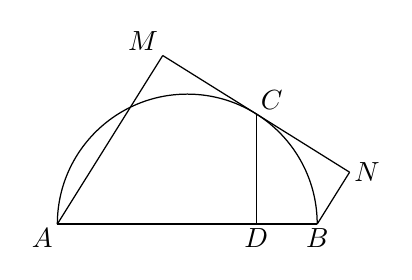
\begin{tikzpicture}[scale=1.65, line width=0.45pt,
  every node/.style={inner sep=1.5pt}]
  \coordinate (A) at (-1,0);
  \coordinate (B) at (1,0);
  \coordinate (C) at (0.53,0.848);
  \coordinate (D) at (0.53,0);
  \coordinate (M) at (-0.189,1.297);
  \coordinate (N) at (1.249,0.399);
  \draw (A) arc (180:0:1);
  \draw (A) -- (B);
  \draw (M) -- (N);
  \draw (A) -- (M);
  \draw (B) -- (N);
  \draw (C) -- (D);
  \node[anchor=south east] at (M) {$M$};
  \node[anchor=south west] at (C) {$C$};
  \node[anchor=west] at (N) {$N$};
  \node[anchor=north east] at (A) {$A$};
  \node[anchor=north] at (D) {$D$};
  \node[anchor=north] at (B) {$B$};
\end{tikzpicture}
